\documentclass[11pt,a4paper]{article}
\usepackage[margin=2.2cm]{geometry}
\usepackage{lmodern}
\usepackage[T1]{fontenc}
\usepackage{microtype}
\usepackage{amsmath,amssymb,bm,mathtools}
\usepackage{booktabs,array}
\usepackage[dvipsnames]{xcolor}
\usepackage{tikz}
\usepackage[most]{tcolorbox}
\usepackage{listings}
\usepackage{enumitem}
\usepackage[colorlinks=true,linkcolor=MidnightBlue,urlcolor=MidnightBlue]{hyperref}
\setlength{\parskip}{5pt}\setlength{\parindent}{0pt}
\setlist{itemsep=2pt,topsep=3pt}
\usetikzlibrary{arrows.meta}

\lstset{language=Python,basicstyle=\ttfamily\small,columns=fullflexible,keepspaces=true,
  keywordstyle=\color{MidnightBlue},commentstyle=\color{gray},showstringspaces=false,frame=none,
  aboveskip=4pt,belowskip=4pt}

\newtcolorbox{plainbox}{colback=blue!4,colframe=MidnightBlue,title=In plain words,fonttitle=\bfseries\small,boxrule=0.6pt,arc=2pt,breakable}
\newtcolorbox{watchbox}{colback=orange!6,colframe=BurntOrange,title=Watch out,fonttitle=\bfseries\small,boxrule=0.6pt,arc=2pt,breakable}
\newtcolorbox{oursbox}{colback=green!5,colframe=ForestGreen,title=In your code,fonttitle=\bfseries\small,boxrule=0.6pt,arc=2pt,breakable}
\newtcolorbox{examplebox}{colback=gray!6,colframe=gray!60,title=Worked example,fonttitle=\bfseries\small,boxrule=0.6pt,arc=2pt,breakable}
\newtcolorbox{whybox}{colback=violet!4,colframe=violet!60!black,title=Why it is true,fonttitle=\bfseries\small,boxrule=0.6pt,arc=2pt,breakable}

\newcommand{\vect}[1]{\mathbf{#1}}
\newcommand{\R}{\mathbb{R}}
\newcommand{\T}{^{\top}}
\newcommand{\vP}{\vect{P}}
\newcommand{\vQ}{\vect{Q}}
\newcommand{\vl}{\vect{l}}
\newcommand{\vm}{\vect{m}}
\newcommand{\vX}{\vect{X}}

\title{\textbf{Homogeneous coordinates, from the ground up}\\[3pt]
\large Where they come from, how three numbers describe points and lines,\\
why the dot and cross products do what they do, and how this runs your Voronoi clipping}
\date{Written for the GNSS-denied whoop swarm project, November 2026}

\begin{document}
\maketitle
\vspace{-1em}
\begin{center}
\begin{minipage}{0.9\textwidth}\small
\textbf{How to read this.} Go in order: each section uses the one before. The two ideas that matter most are in
Section~\ref{sec:dot} (dot product: is the point on the line, and on which side) and Section~\ref{sec:cross} (cross
product: join two points, meet two lines). Section~\ref{sec:clip} puts them together in your \texttt{create\_cells}.
A note on the name: what you want is \emph{homogeneous coordinates}, also called the \emph{projective plane}.
``Homogeneous space'' is a different, advanced topic in group theory, so search for the first two terms.
\end{minipage}
\end{center}

\tableofcontents

%==========================================================================================
\section{The problem they solve}

In ordinary coordinates a line and a point are different kinds of object, and intersecting two lines needs a formula
with special cases. The line $y=mx+k$ cannot even describe a vertical line. The form $ax+by+c=0$ can, so use that.
Now solve two of them together, and you get (Cramer's rule)
\[
x=\frac{b_1c_2-b_2c_1}{a_1b_2-a_2b_1},\qquad y=\frac{c_1a_2-c_2a_1}{a_1b_2-a_2b_1}.
\]
Look at the shape of this. Three numbers appear: two numerators and one shared denominator. Parallel lines make the
denominator zero, which in ordinary coordinates is a crash.

Homogeneous coordinates keep those three numbers \emph{without doing the division}. Then:
\begin{itemize}
\item a point and a line are both just three numbers;
\item ``is this point on this line?'' is a dot product;
\item ``the line through two points'' and ``the point where two lines meet'' are both a cross product;
\item parallel lines are no longer a special case: they meet at a point with $w=0$;
\item moving, scaling and squishing all become one matrix multiplication.
\end{itemize}

%==========================================================================================
\section{Where they come from}

The idea comes from perspective drawing. Stand on a railway line: the rails are parallel, yet in a photograph they meet at
a point on the horizon. Painters worked this out in the Renaissance. Mathematicians then made it exact, and homogeneous
coordinates were introduced by M\"obius in 1827.

The picture to keep in your head is a pinhole camera. Your eye is the origin of 3D space, and in front of it, at height
$w=1$, is a flat sheet of glass: your 2D world. Every ray from the eye that hits the glass marks exactly one point on it.

\begin{center}
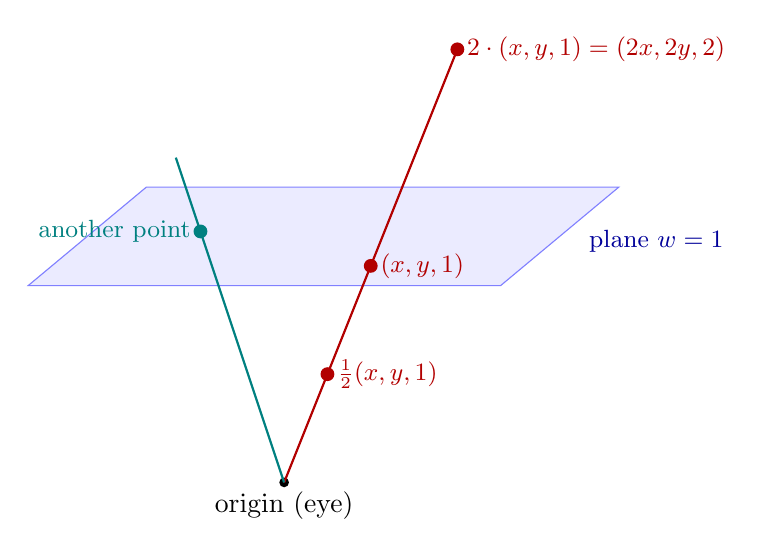
\begin{tikzpicture}[scale=1.25,>=Latex]
\fill[blue!8] (-2.6,2)--(2.2,2)--(3.4,3)--(-1.4,3)--cycle;
\draw[blue!50] (-2.6,2)--(2.2,2)--(3.4,3)--(-1.4,3)--cycle;
\node[blue!60!black,font=\small,anchor=west] at (3.0,2.45) {plane $w=1$};
\fill (0,0) circle (1.4pt) node[below]{origin (eye)};
\draw[thick,red!70!black] (0,0)--(1.76,4.4);
\fill[red!70!black] (0.88,2.2) circle (2pt) node[right,font=\small]{$(x,y,1)$};
\fill[red!70!black] (1.76,4.4) circle (2pt) node[right,font=\small]{$2\cdot(x,y,1)=(2x,2y,2)$};
\fill[red!70!black] (0.44,1.1) circle (2pt) node[right,font=\small]{$\tfrac12(x,y,1)$};
\draw[thick,teal] (0,0)--(-1.1,3.3);
\fill[teal] (-0.85,2.55) circle (2pt) node[left,font=\small]{another point};
\end{tikzpicture}
\end{center}

\begin{plainbox}
A 2D point \emph{is} a ray through the origin of 3D. Any 3D point on that ray names the same 2D point. The vector
$(x,y,w)$ with $w\ne0$ hits the glass at $(x/w,\,y/w)$. That one sentence is the whole definition.
\end{plainbox}

%==========================================================================================
\section{Points}

A 2D point $(x,y)$ is written as $(x,y,1)$. Scaling by any non-zero number gives the same point:
\[
(x,y,w)\sim(\lambda x,\lambda y,\lambda w),\qquad \lambda\ne0,
\qquad\text{and back to ordinary coordinates: }(x,y,w)\mapsto(x/w,\;y/w).
\]
This is the word \emph{homogeneous}: overall scale does not matter. So $(1,2,1)$, $(2,4,2)$ and $(-3,-6,-3)$ are the same
point, and only the ratios count. Note that $w$ can be negative. Three numbers but only two degrees of freedom.

\textbf{What if $w=0$?} The ray $(x,y,0)$ is flat, parallel to the glass, and never hits it. It is a
\emph{point at infinity}, and it means a direction: $(1,0,0)$ is ``far away in the $x$ direction''.
Only $(0,0,0)$ is forbidden, because it isn't a ray.

\begin{oursbox}
\begin{lstlisting}
poly_h = np.column_stack([q_w, np.ones(len(q_w))])   # (x, y) -> (x, y, 1)
q      = poly_h[:, :2] / poly_h[:, 2:]               # general way back
\end{lstlisting}
If every row already has $w=1$, then \texttt{poly\_h[:, :2]} is enough.
\end{oursbox}

%==========================================================================================
\section{Lines}

A line is also three numbers, $\vl=(a,b,c)$, meaning all points with $ax+by+c=0$. Multiplying the equation by $\lambda\ne0$
doesn't change which points satisfy it, so lines are homogeneous too: $(1,1,-3)$ and $(2,2,-6)$ are the same line.

Geometrically, the line on the glass together with the eye spans a \emph{plane through the origin}, and a plane through the
origin is described by its normal. That normal is $\vl$.

\begin{center}
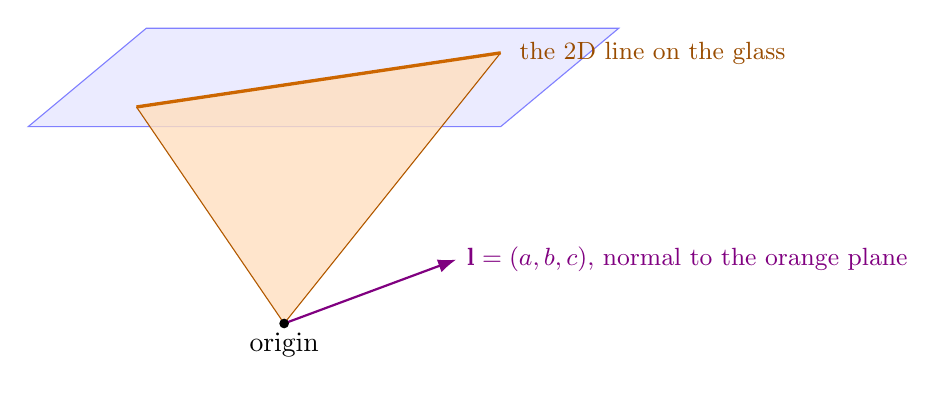
\begin{tikzpicture}[scale=1.25,>=Latex]
\fill[blue!8] (-2.6,2)--(2.2,2)--(3.4,3)--(-1.4,3)--cycle;
\draw[blue!50] (-2.6,2)--(2.2,2)--(3.4,3)--(-1.4,3)--cycle;
\fill[orange!25,opacity=.8] (0,0)--(-1.5,2.2)--(2.2,2.75)--cycle;
\draw[orange!70!black] (0,0)--(-1.5,2.2);
\draw[orange!70!black] (0,0)--(2.2,2.75);
\draw[very thick,orange!80!black] (-1.5,2.2)--(2.2,2.75);
\node[orange!60!black,font=\small] at (3.7,2.75) {\ the 2D line on the glass};
\draw[->,thick,violet] (0,0)--(1.75,0.65) node[right,font=\small]{$\vl=(a,b,c)$, normal to the orange plane};
\fill (0,0) circle (1.4pt) node[below]{origin};
\end{tikzpicture}
\end{center}

What the three numbers mean, when the line is written $ax+by+c=0$:
\begin{itemize}
\item $(a,b)$ is a normal of the line in 2D: it is perpendicular to the line.
\item $c$ sets how far the line is from the origin: the distance is $|c|/\|(a,b)\|$.
\item $\vl$ and $-\vl$ are the same line, but they have opposite normals. This matters in the next section.
\item $(0,0,1)$ is the \emph{line at infinity}: the set of all points with $w=0$.
\end{itemize}

%==========================================================================================
\section{The dot product: on the line, and on which side}\label{sec:dot}

Take a point $\vP=(x,y,1)$ and a line $\vl=(a,b,c)$. Their dot product is
\[
s=\vl\cdot\vP=ax+by+c .
\]
This is the line equation with the point put in, so:

\begin{center}
\begin{tabular}{ll}
\toprule
$s=0$ & the point is on the line\\
$s<0$ & one side\\
$s>0$ & the other side\\
\bottomrule
\end{tabular}
\end{center}

In the 3D picture, $\vl\cdot\vP=0$ says the ray is perpendicular to the normal, so it lies inside the orange plane.

\textbf{Why does the sign give the side?} Pick any point $\vect{x}_0$ on the line, so $\vect{n}\cdot\vect{x}_0+c=0$, where
$\vect{n}=(a,b)$. Then for any $\vect{x}$:
\[
s=\vect{n}\cdot\vect{x}+c=\vect{n}\cdot(\vect{x}-\vect{x}_0)=\|\vect{n}\|\;\times\;\text{(signed distance from the line)}.
\]
A dot product with $\vect{n}$ measures how far you've gone in the direction of $\vect{n}$. So $s$ is positive on the side
$\vect{n}$ points to, and $s/\|\vect{n}\|$ is the true signed distance.

\begin{whybox}
\textbf{For your bisector}, $\vect{n}=\vect{p}_j-\vect{p}_i$ and $c=-\tfrac12(\|\vect{p}_j\|^2-\|\vect{p}_i\|^2)$. Expand:
\[
\tfrac12\big(\|\vect{x}-\vect{p}_i\|^2-\|\vect{x}-\vect{p}_j\|^2\big)
=\tfrac12\big(-2\vect{x}\cdot\vect{p}_i+\|\vect{p}_i\|^2+2\vect{x}\cdot\vect{p}_j-\|\vect{p}_j\|^2\big)
=\vect{x}\cdot\vect{n}+c=s.
\]
The $\|\vect{x}\|^2$ terms cancelled, which is why a bisector is straight. And $s<0$ means exactly that $\vect{x}$ is closer
to drone $i$.
\end{whybox}

\begin{examplebox}
Drones at $\vect{p}_i=(0,0)$ and $\vect{p}_j=(2,0)$. Then $\vect{n}=(2,0)$, $c=-2$, so $\vl=(2,0,-2)$: the line $x=1$.
At $(0,0)$: $s=-2$, closer to $i$. At $(3,1)$: $s=4$, and indeed $\tfrac12(10-2)=4$, closer to $j$.
\end{examplebox}

\begin{watchbox}
The side test needs \textbf{a sign convention you control}.
\begin{itemize}
\item $-\vl$ is the same line, but flips the sign of every $s$. So build side-test lines from $\vect{n}$ and $c$.
\item With a general $w$, $\vl\cdot(x,y,w)=w\cdot s$. A negative $w$ flips the sign, and any $w\neq1$ scales it. Keep $w=1$ for
vertices. For ``on the line?'' only ($s=0$), neither of these matters.
\end{itemize}
\end{watchbox}

%==========================================================================================
\section{The cross product: join and meet}\label{sec:cross}

For 3-vectors,
\[
\vect{u}\times\vect{v}=\big(u_2v_3-u_3v_2,\;\;u_3v_1-u_1v_3,\;\;u_1v_2-u_2v_1\big).
\]
The one fact that matters: \textbf{the result is perpendicular to both inputs}.
\begin{whybox}
$\vect{a}\cdot(\vect{u}\times\vect{v})$ equals the determinant with rows $\vect{a},\vect{u},\vect{v}$. A determinant with two equal
rows is zero. So $\vect{u}\cdot(\vect{u}\times\vect{v})=0$ and $\vect{v}\cdot(\vect{u}\times\vect{v})=0$.
\end{whybox}

\textbf{Line through two points (join).} We want $\vl$ with $\vl\cdot\vP=0$ and $\vl\cdot\vQ=0$, so $\vl$ must be perpendicular
to both $\vP$ and $\vQ$. That is what the cross product makes:
\[
\vl=\vP\times\vQ .
\]
\textbf{Point on two lines (meet).} We want $\vX$ with $\vl\cdot\vX=0$ and $\vm\cdot\vX=0$. It's the same equation with the
roles swapped:
\[
\vX=\vl\times\vm .
\]

\begin{center}
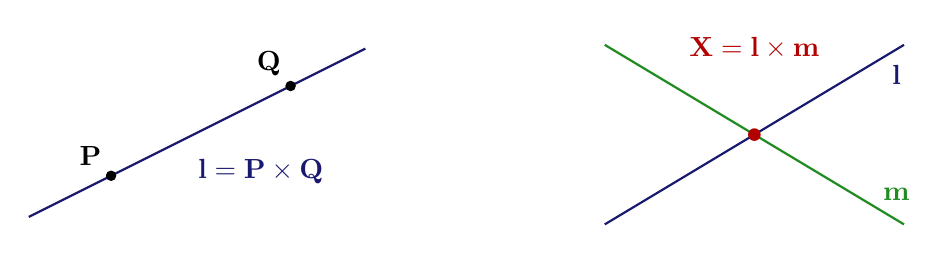
\begin{tikzpicture}[scale=0.95,>=Latex]
\begin{scope}
\draw[thick,MidnightBlue] (-0.5,0.1)--(4,2.35);
\fill (0.6,0.65) circle (2pt) node[above left]{$\vP$};
\fill (3,1.85) circle (2pt) node[above left]{$\vQ$};
\node[MidnightBlue] at (2.6,0.7) {$\vl=\vP\times\vQ$};
\end{scope}
\begin{scope}[xshift=7.2cm]
\draw[thick,MidnightBlue] (0,0)--(4,2.4);
\draw[thick,ForestGreen] (0,2.4)--(4,0);
\fill[red!70!black] (2,1.2) circle (2.4pt) node[above=24pt]{$\vX=\vl\times\vm$};
\node[MidnightBlue] at (3.9,2.0) {$\vl$};
\node[ForestGreen] at (3.9,0.4) {$\vm$};
\end{scope}
\end{tikzpicture}
\end{center}

\begin{plainbox}
Points and lines swap roles with no change in the maths. This is called \emph{duality}: any true statement about points and
lines stays true if you swap the two words. One operation does both jobs.
\end{plainbox}

\begin{examplebox}
\textbf{Join.} $\vP=(1,2,1)$, $\vQ=(3,3,1)$ gives $\vl=(2\cdot1-1\cdot3,\;1\cdot3-1\cdot1,\;1\cdot3-2\cdot3)=(-1,2,-3)$.
Check: $-1+4-3=0$ and $-3+6-3=0$.

\textbf{Meet.} $x+y-3=0$ and $x-y-1=0$: $\vl=(1,1,-3)$, $\vm=(1,-1,-1)$, so $\vl\times\vm=(-4,-2,-2)$. Divide by $w=-2$:
the point $(2,1)$. Check: $2+1=3$ and $2-1=1$.
\end{examplebox}

\textbf{It is Cramer's rule.} Write out $\vl\times\vm$ for $\vl=(a_1,b_1,c_1)$ and $\vm=(a_2,b_2,c_2)$:
\[
\vl\times\vm=\big(\,b_1c_2-b_2c_1,\;\;c_1a_2-c_2a_1,\;\;a_1b_2-a_2b_1\,\big).
\]
Those are the two numerators and the denominator from Section~1, in order. The division by $w$ is the division in Cramer's
rule, just done later.

\textbf{Parallel lines.} The third number is $w=a_1b_2-a_2b_1$, which is the 2D cross product of the two normals. It is zero
exactly when the normals are parallel. So parallel lines meet at $w=0$, a point at infinity.
\begin{examplebox}
$x=1$ and $x=2$: $\vl=(1,0,-1)$, $\vm=(1,0,-2)$, so $\vl\times\vm=(0,1,0)$. That's ``infinitely far in the $y$ direction'',
the direction both lines run in. For the same line twice, the cross product is $(0,0,0)$: no unique answer.
\end{examplebox}

\textbf{The sign of a cross product.} Swapping the inputs flips the sign: $\vP\times\vQ=-\vQ\times\vP$. For a meet point this
is harmless, because dividing by $w$ cancels it. For a line used in a side test, the order decides which side is positive: if
$\vl=\vP\times\vQ$ with $w=1$ points, then
\[
\vl\cdot\vect{R}=\det[\vP,\vQ,\vect{R}]=2\times\text{signed area of triangle }PQR ,
\]
which is positive when $\vect{R}$ is to the \emph{left} of the direction $\vP\to\vQ$. This is the standard orientation test.

%==========================================================================================
\section{Moving things: one matrix for everything}

An ordinary $2\times2$ matrix can rotate and scale, but can't translate, since it always sends $(0,0)$ to $(0,0)$. In
homogeneous coordinates translation becomes a matrix too:
\[
\begin{pmatrix}x'\\y'\\1\end{pmatrix}=
\begin{pmatrix}\multicolumn{2}{c}{\;\;M\;\;}&\begin{matrix}t_x\\t_y\end{matrix}\\[2pt]0&0&1\end{pmatrix}
\begin{pmatrix}x\\y\\1\end{pmatrix},
\qquad \vect{x}'=M\vect{x}+\vect{t}.
\]
In the 3D picture, this is a \emph{shear}, which is linear. Translation looks non-linear on the glass, but it's linear
in the space above it. Chaining motions is now just multiplying matrices.

\begin{oursbox}
Your DVS map $\vect{q}_w=\vect{p}_W+r\,A\,\vect{q}_b$ is one matrix:
\[
H=\begin{pmatrix}rA&\vect{p}_W\\ \vect{0}\T&1\end{pmatrix},\qquad A=\mathrm{diag}(\alpha,1/\alpha).
\]
\end{oursbox}

\textbf{Lines transform differently.} If points move by $\vect{x}'=H\vect{x}$, lines move by $\vl'=H^{-\top}\vl$.
\begin{whybox}
The new line must still contain the moved points: $\vl'\cdot\vect{x}'=\vl'^{\top}H\vect{x}$ must equal $\vl\T\vect{x}$. That needs
$\vl'^{\top}H=\vl\T$, so $\vl'=H^{-\top}\vl$.
\end{whybox}
\begin{examplebox}
Translate by $(2,3)$. The line $x=1$ is $(1,0,-1)$, and $H^{-\top}$ gives $(1,0,-3)$: the line $x=3$. Correct.
\end{examplebox}

\begin{watchbox}
A matrix sends a line to a line, but not a bisector to a bisector, unless it preserves angles and ratios. Squish the plane by
$A$ and the squished bisector is no longer perpendicular to the squished drones. That's why you recompute cells from the real
drone positions every step, rather than transforming old ones.
\end{watchbox}

%==========================================================================================
\section{Clipping: your code, line by line}\label{sec:clip}

Here is one clip of the polygon \texttt{poly} by a bisector \texttt{l}:
\begin{lstlisting}
s = poly @ l                                # dot product: side of each vertex
keep = []
for k in range(len(poly)):
    m = (k + 1) % len(poly)                 # next vertex
    if s[k] <= 0:                           # keep our side
        keep.append(poly[k])
    if s[k] * s[m] < 0:                     # this edge crosses l
        e = np.cross(poly[k], poly[m])      # join: the edge's line
        X = np.cross(l, e)                  # meet: edge line x bisector
        keep.append(X / X[2])               # back to w = 1
poly = np.array(keep).reshape(-1, 3)
\end{lstlisting}

\begin{center}
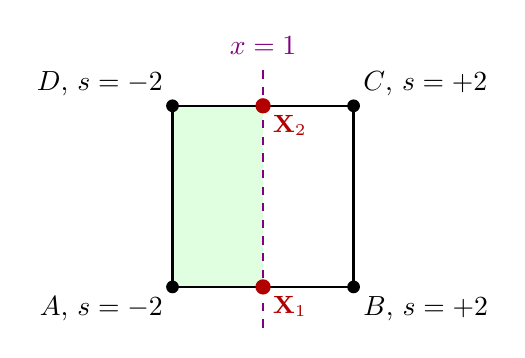
\begin{tikzpicture}[scale=1.15,>=Latex]
\fill[green!12] (0,0)--(1,0)--(1,2)--(0,2)--cycle;
\draw[thick] (0,0)--(2,0)--(2,2)--(0,2)--cycle;
\draw[dashed,violet,thick] (1,-0.45)--(1,2.45) node[above]{$x=1$};
\fill (0,0) circle (2pt) node[below left]{$A$, $s=-2$};
\fill (2,0) circle (2pt) node[below right]{$B$, $s=+2$};
\fill (2,2) circle (2pt) node[above right]{$C$, $s=+2$};
\fill (0,2) circle (2pt) node[above left]{$D$, $s=-2$};
\fill[red!70!black] (1,0) circle (2.4pt) node[below right,font=\small]{$\vX_1$};
\fill[red!70!black] (1,2) circle (2.4pt) node[below right,font=\small]{$\vX_2$};
\end{tikzpicture}
\end{center}

\begin{examplebox}
Square $A(0,0)$, $B(2,0)$, $C(2,2)$, $D(0,2)$, cut by $\vl=(2,0,-2)$. The walk keeps $A$; $A\to B$ changes sign, so add $\vX_1$;
$B,C$ are dropped; $C\to D$ changes sign, so add $\vX_2$; keep $D$. Result: $A,\vX_1,\vX_2,D$, in order.

$\vX_1$: $\vect{e}=A\times B=(0,2,0)$, then $\vl\times\vect{e}=(4,0,4)$, so the point is $(1,0)$.

$\vX_2$: $\vect{e}=C\times D=(0,-2,4)$, then $\vl\times\vect{e}=(-4,-8,-4)$, so the point is $(1,2)$. Here $w=-4$:
a real example of why you divide before storing.
\end{examplebox}

\subsection*{The neat identity: the cross product already knows $s$}
The vector identity $\vect{a}\times(\vect{b}\times\vect{c})=\vect{b}(\vect{a}\cdot\vect{c})-\vect{c}(\vect{a}\cdot\vect{b})$ gives, for an edge $\vP\to\vQ$ with $w=1$:
\[
\vl\times(\vP\times\vQ)=\vP\,(\vl\cdot\vQ)-\vQ\,(\vl\cdot\vP)=s_Q\vP-s_P\vQ .
\]
The third component gives $w=s_Q-s_P$. Dividing:
\[
\frac{s_Q\vP-s_P\vQ}{s_Q-s_P}=(1-t)\vP+t\vQ,\qquad t=\frac{s_P}{s_P-s_Q}.
\]
This shows three things:
\begin{itemize}
\item The homogeneous version and the \texttt{t} version are \textbf{the same formula}.
\item If $s_P$ and $s_Q$ have opposite signs, then $w=s_Q-s_P\ne0$. That's the reason you can never divide by zero after the
\texttt{s[k]*s[m]<0} test.
\item $0<t<1$, so the crossing is really between $\vP$ and $\vQ$, and never far away.
\end{itemize}

\subsection*{Why you never get a wrong vertex}
The value $s$ of any line is linear, so for $\vX=(1-t)\vP+t\vQ$, and any earlier bisector $\vl_1$:
\[
s_1(\vX)=(1-t)\,s_1(\vP)+t\,s_1(\vQ)\le 0
\quad\text{when } s_1(\vP)\le0 \text{ and } s_1(\vQ)\le0 .
\]
New crossings stay valid for all earlier cuts, and later cuts test them as ordinary vertices. An edge created by an earlier cut
lies on that bisector, so \texttt{np.cross(poly[k], poly[m])} rebuilds it, and the same line of code also finds where two
bisectors meet.

%==========================================================================================
\section{Traps when you compute with this}

\begin{center}
\begin{tabular}{p{0.42\textwidth}p{0.48\textwidth}}
\toprule
\textbf{Trap} & \textbf{What to do}\\
\midrule
A vertex stored with $w\ne1$ & Divide when you create it, or the next $s$ is scaled or flipped.\\
Side test on a line made by a cross product & Sign depends on point order. Build from $\vect{n},c$, or fix the order.\\
Comparing $w$ with exactly 0 & Rounding means $w\approx10^{-16}$. Use a tolerance, or test signs first as clipping does.\\
Numbers growing after repeated crosses & Divide by $w$, or by $\|\vl\|$, so they stay near 1.\\
Comparing two lines with \texttt{==} & $(1,1,-3)$ and $(2,2,-6)$ are equal. Test $\|\vl\times\vm\|\approx0$.\\
Using $s$ as a distance & Divide by $\|(a,b)\|$ first. Your $s$ is distance times $\|\vect{p}_j-\vect{p}_i\|$.\\
\bottomrule
\end{tabular}
\end{center}

%==========================================================================================
\section{A few more things worth knowing}

\begin{itemize}
\item \textbf{Three points on one line:} $\det[\vP,\vQ,\vect{R}]=0$. \textbf{Three lines through one point:} the same with lines.
\item \textbf{Projective maps:} a general $3\times3$ matrix with a non-trivial bottom row is a \emph{homography}. It can bring
points at infinity into view, which is the railway picture. It keeps lines straight, but not parallelism. Four point pairs
determine it.
\item \textbf{Cameras:} a pinhole camera is $\vect{x}\sim K[R\mid\vect{t}]\vect{X}$: 3D homogeneous point in, 2D homogeneous point
out, and the divide by $w$ is the perspective divide. If you add an overhead camera to the whoops, this is the formula.
\item \textbf{3D:} points become $(x,y,z,1)$, and planes $(a,b,c,d)$ work like lines do here. Rigid motions are $4\times4$ matrices,
as in ROS and robotics generally. The cross-product shortcuts do not carry over directly: 3D lines need more machinery.
\item \textbf{Conics:} a circle or ellipse is $\vect{x}\T C\,\vect{x}=0$ for a symmetric $3\times3$ matrix $C$, and moves by
$C'=H^{-\top}CH^{-1}$.
\item \textbf{Why you may not need them:} for one line and one edge, the \texttt{t} formula is just as short. Homogeneous form earns
its place when you do many joins and meets, chain transforms, or work with cameras.
\end{itemize}

%==========================================================================================
\section{Cheat sheet}

\begin{center}
\renewcommand{\arraystretch}{1.25}
\begin{tabular}{ll}
\toprule
\textbf{Question} & \textbf{Answer}\\
\midrule
Point to homogeneous & $(x,y)\to(x,y,1)$\\
Back to ordinary & $(x/w,\;y/w)$\\
Same point / same line & equal up to a non-zero scale\\
Point on line? & $\vl\cdot\vP=0$\\
Which side? & sign of $\vl\cdot\vP$ with $w=1$\\
Signed distance & $\vl\cdot\vP/\|(a,b)\|$ with $w=1$\\
Line through two points & $\vl=\vP\times\vQ$\\
Point on two lines & $\vX=\vl\times\vm$, then divide by $w$\\
Parallel lines & $w=0$\\
Bisector of drones $i,j$ & $\big(p_j-p_i,\;-\tfrac12(\|p_j\|^2-\|p_i\|^2)\big)$\\
Transform points & $\vect{x}'=H\vect{x}$\\
Transform lines & $\vl'=H^{-\top}\vl$\\
\bottomrule
\end{tabular}
\end{center}

%==========================================================================================
\section{Try it yourself}

Do these by hand, then check with \texttt{np.cross}.
\begin{enumerate}
\item Are $(1,2,1)$ and $(-2,-4,-2)$ the same point? What ordinary point is $(6,3,3)$?
\item Find the line through $(0,0)$ and $(1,1)$. Is $(2,2)$ on it? On which side is $(0,1)$?
\item Where do $y=1$ and $x=3$ meet?
\item Where do $y=x$ and $y=x+1$ meet? What does the answer mean?
\item Drones at $(0,0)$ and $(0,4)$: write the bisector as $(a,b,c)$. Which side is $(5,1)$ on, and what is its distance from the bisector?
\item Clip the square of Section~\ref{sec:clip} with $x+y-3=0$, keeping $x+y-3\le0$. List the vertices in order.
\end{enumerate}

\textbf{Answers.}
\begin{enumerate}[itemsep=1pt]
\item Yes ($\lambda=-2$). $(2,1)$.
\item $(0,0,1)\times(1,1,1)=(-1,1,0)$, so $y=x$. Yes: $-2+2=0$. $(0,1)$ gives $s=1>0$, the left of the direction $(0,0)\to(1,1)$.
\item $(0,1,-1)\times(1,0,-3)=(-3,-1,-1)$, so the point $(3,1)$.
\item $(1,-1,0)\times(1,-1,1)=(-1,-1,0)$: $w=0$, so they're parallel, and they meet at infinity in the direction $(1,1)$.
\item $\vect{n}=(0,4)$, $c=-8$, so $(0,4,-8)$, the line $y=2$. $s=4-8=-4<0$: closer to the drone at $(0,0)$. Distance $4/4=1$.
\item $s$ for $A,B,C,D$ is $-3,-1,+1,-1$. Result: $A$, $B$, $(2,1)$, $(1,2)$, $D$.
\end{enumerate}

\end{document}
